\documentclass[journal]{IEEEtran}


\usepackage[czech]{babel}


% DOPLNIJICI BALICKY
\usepackage[utf8]		%	Kódování zdrojových souborů je Windows-1250
	{inputenc}					% Balíček pro nastavení kódování zdrojových souborů
\usepackage{cmap} 		% Balíček cmap zajišťuje, že PDF vytvořené `pdflatexem' je
											% plně "prohledávatelné" a "kopírovatelné"

\usepackage{amsmath}
\usepackage{caption}
\usepackage{dsfont}
\usepackage{layouts}
\usepackage{graphicx}
\usepackage{hyperref}
\usepackage{subcaption}
\usepackage{acro}
\usepackage{listings}

\include{ac}


\def\contentsname{Contents}
\def\listfigurename{List of Figures}
\def\listtablename{List of Tables}
\def\refname{References}
\def\indexname{Index}
\def\figurename{Obr.}
\def\tablename{Tab.}
\def\partname{Part}
\def\appendixname{Appendix}
\def\abstractname{Abstract}
% IEEE specific names
\def\IEEEkeywordsname{Klíčová slova}
\def\IEEEproofname{Proof}



% zkratky
\DeclareAcronym{MSE}{
  short=MSE,
  long=mean squared error
}

\DeclareAcronym{PSNR}{
  short=PSNR,
  long=peak signal-to-noise ratio
}

\DeclareAcronym{SSIM}{
  short=SSIM,
  long=structural similarity
}
% konec zkratek


\title{Klasifikace obrazu }


\author{Ondře Rajnet
        \linebreak
        Faculty of Informatics and Management
        \linebreak
        University of Hradec Kralove,
        \linebreak
        Hradec Kralove, Czech Republic
        \linebreak
        rajneon1@uhk.cz

}

\begin{document}

% make the title area
\maketitle

% As a general rule, do not put math, special symbols or citations
% in the abstract or keywords.
\begin{abstract}

Tato práce se zabývá problematikou strojového učení. V dnešní době, je stále více a více roste obliba umělé inteligence a strojového učení. Aplikace, která bude sloužit jako demonstrace strojového učení, je zaměřena především na rozpoznání obrazu, konkrétně na rozpoznání nemocí (vředy, vaskulární onemocnění, …) na obrazu a jejich následné vyhodnocení, zda je nebo není nemoc přítomná. Budeme náš model postupně cvičit a trénovat pro lepší a přesnější výsledky. Používat nebudeme jenom jeden model, pro učení, ale vyzkoušíme jich více a porovnáme výsledky, které jednotlivý model přináší.

\end{abstract}

% Note that keywords are not normally used for peerreview papers.
\begin{IEEEkeywords}
Inception-v3 1; rozpoznání obrazu 2; strojové učení 3; neuronové sítě 4;umělá inteligence 5;
\end{IEEEkeywords}


\IEEEpeerreviewmaketitle



\section{ÚVOD}

\subsection{OBSAH}
V dnešní moderní době roste velikým tempem popularita strojového učení. Může za to dnešní doba a rozšíření mobilních telefonů mezi masu lidí. Tím, že každý z nás využívá chytrý mobilní telefon, tak možná nevědomky přispívá k umělé inteligenci. Tito uživatelé poskytují obrovské množství dat, které se dají využít pro trénování strojového učení.
Nemusíme chodit ani nikam daleko, podívejme se na Iphony a jejich funkci “Deep fusion” [1]. Tuto funkci představil Apple v roce 2019 pro na vylepšení fotografií pořízených pomocí mobilního telefonu. Funkce využívá “neural enginu” [2], který má v sobě zabudovaný přímo procesor a s jeho pomocí vylepšuje fotografie.

Hlavním cílem této práce je vytvoření funkčního modelu, pro rozpoznání obrazu. Model bude vycházet ze zadaného datasetu. Dataset se postupně zpracuje a natrénuje pro aktuální použití. V našem případě budeme rozpoznávat nemoci. Po natrénovaní budeme schopni používat obrazy a rozpoznávat na nich případné nemoci. Bude to usnadnění pro lidi, kteří to nemusí rozpoznávat pomocí odborníků. Samozřejmě model nebude přesný na 100 procent, ale posouží nám jako orientační hodnota.

Strojové učení (ML) je jeden z typů umělé inteligence (AI), který umožnuje aplikacím přinést přesnější a lepší předpovědi výsledků a nemusí k tomu být úplně přímo naprogramovaný. ML využívá historická data pro svůj vstup k předpovědi výstupních hodnot. [3]

Strojové učení mám pod sebou velice silné případy použití, od předvídaní chování zákazníků při nákupech. Mezi výhody můžeme zařadit pomoc porozumět svým zákazníkům na hlubší úrovni. Hromaděním informací o svých zákaznících a jejich korelací v průběhu času. S přibývajícími daty a časem se algoritmy strojového učení naučí asociaci a pomáhat přizpůsobit vývoj produktu nebo v oblasti marketingu mají obrovský potenciál. 
Už se objevili velké internetové společnosti, které využívají strojové učení jako hlavní sílu ve svých obchodních modelech. Můžeme si říci pár příkladů. Společnosti Uber využívá algoritmy k porovnání řidičů. Google využívá strojové učení k zobrazování cílené reklamy na správného zákazníka. 
Samozřejmě, není to jen tak, že strojové učení by mělo samé výhody. Jedna z prvních překážek může být cena za daný projekt. Projekty tohoto typu, řídí lidé, kteří jsou datový vědci a odborníci na svých místech, a to odpovídá jejich platům. Také je vyžadována vysoká softwarová infrastruktura. 
Dále může být v zaujatosti algoritmů. Data, která dostaneme od určité populace nebo v data obsahují nějaké chyby vedou k nepřesním modelům světa. Tyto modely v lepším případě selžou v horších případech jsou diskriminační. Podnik může založit základní obchodní procesy na neobjektivních modelech, může dojít k poškození reputace a tím zmaření podnikání. [3] 

Algoritmy strojového učení jsou s námi už více než deset let, až nyní získali novou popularitu, protože se stále více do života dostává uměla inteligence. Modely hlubokého učení (Deep learning) podporují nejmodernější aplikace současné doby. 
Platformy ML patří v současností mezi nejkonkurenceschopnější oblasti podnikových technologií. Většina velkých výrobců softwaru (Google, Microsoft, IBM) bojují o přihlášení uživatele právě na jejich platformu. Tyto platformy pokrývají obrovské spektrum činností strojového učení, dají se sbírat data, vyhodnocovat, vytvářet modely, klasifikace dat. 
Strojové učení bude mít v životě lidí větší a větší důležitost. Nejen pro obyčejného zákazníka, ale hlavně pro firmy. Bitvy o data zákazníků můžeme vidět již dneska, tato válka se bude jen dále prohlubovat. [3]

\section{PROBLEM DEFINITION/ DEFINICE PROBLÉMU}
\subsection{OBSAH}
V oblasti pro rozpoznání obrazu je mnoho modelů které se dají implemenovat. Modelů je více a proto je dobré si je porovnat. Porovnání výběru modelů můžeme v článcích [4]. Všechny možné řešení, které již jsou, využívají neuronové sítě, ale každá se bude lišit v konkrétní implementaci nad konkrétním případem a nebude existovat univerzální řešení pro všechny.

Typy strojového učení se rozdělují podle toho, jak se algoritmus učí dávat přesnější výsledky. Máme 4 základní algoritmy: učení pod dohledem, učení bez dozoru, učení s částečným dohledem a posilovací učení. Níže si rozebere každý z nich. 
Kontrolované učení, v tomto typu datoví vědci dodávají algoritmům označená tréninková data a definují proměnné, které chtějí, aby algoritmus vyhodnotil pro korelace. Specifikuje se vstup výstup. 
Učení bez dozoru, patří sem algoritmy, které se cvičí na neoznačených datech. Algoritmus pracuje na principu prohledávání datové sady (datasetu) a vyhledávání smysluplné spojení. Předpovědi nebo doporučení na kterých se algoritmy trénují jsou předem učená. 
Učení s částečným dohledem, kombinace předchozím dvou řešení. Vědci mohou algoritmu dávat většinu dat která jsou označená jako tréninková, ale model může data sám volně prozkoumávat a rozbíjet vlastní porozumění datové sadě. 
Posílení učení, využívá učení výztuže, která se většinou používá k naučení algoritmu dokončit vícestupňový proces. Pro tento proces existují jasně definovaná pravidla. Algoritmus je naprogramován tak, aby splnil úkol a dostal pozitivní nebo negativní podmět, když zjistí, jak ho dokončit. Jaké kroky podnikne se většinou algoritmus rozhoduje sám. [3]

Hlavní vize celé této práce je rozpoznání obrazu nad obrazy onemocnění, které budou zanesení do datasetu a následně s tímto datasetem budeme pracovat. 

V odborné práci [5] se autoři zabývají obrazy mozku. Zkoumají oblasti CT v moderním počítačovém podání. Hlavním jejich oblast zkoumání je zda může konvoluční neuronové sítě (CNN) poskytnout doplňující informace ohledně včasné diagnostiky Alzheimerovy choroby. Sestavili 3 kategorie CT snímků AD, Léze (Nádor) a normální stárnutí. Kvůli vlastnostem této korelace a její hloubky je zavedená pokročilá architektura integrující 2D a 3D sítě CNN. Spojení těchto 2 sítí je následně vyhodnocena na základě 2D obrazu podél prostorových axiálních směrů a 3 D segmentovaných bloků. Výsledky této spolupráce s touto neobvyklou propracovanou architekturou poskytují velice vysoká procenta úspěšnosti. 

  

V odborné práci [6] se autoři zabývají předpovědí mrtvice pomocí strojového učení. Při klinickém rozhodování se v praxi uplatňuje mnoho prediktivních technik, které lékařům pomáhají s určením diagnozy a léčby pacientů. Konvekční prediktivní modely nebo techniky jsou však stále nedostateční, a proto se rozhodli udělat tento výzkum. Tato práce uvádí techniky pro cévní mozkovou příhodu aplikovanou na dataset srdečních chorob. Příznaky fibrilace síní u pacientů jsou hlavním rizikovým faktore cévní mozkové příhody. Výsledkem výzkumu je přesnější skórovací systém, které se v současné době používá pro varování pacientů, u kterých je pravděpodobné, že u nich může dojít k mrtvici. 

  

V článku [7], je provedená studie, která se zabývá předpovědí oční axiální délky na základě vizuální interpretace obrazů sítnicového pozadí. Oční axiální délka (Al) je důležitou vlastní očí používaných ke stanovení zdraví před operací pacienta. Zásadní při je Al při výrobě umělých čoček, které nahrazují poškozené oční čočky, která má pacient. Přesně měření je však velice náročné a nákladné. Dnešní moderní fotoaparáty jsou na takové úrovní, a tak dokáži zachytit složitou strukturu očí fundus. Kvůli se tomu se rozhodli na nákladě těchto snímků vyzkoušet hlubokého učení. S přispěním vizualizační techniky lze lokalizovat diskriminační oblasti zájmu pro předpovědi. V experimentu bylo zjištěn významný vtah mezi fundusem a Al s dosaženým koeficientem s přesností 90 procent. Výsledná neurovnová síť předpovídá Al konzistentní oblasti. Výsledek této studie dokazuje souvislost mezi Al a biologickou strukturou očí. 



Dnes se můžeme setkat se strojovým učením na e-shopu. V podobě zákaznické podpory, která vám v případě nouze poradí. Na druhé straně, ale nemusí být nějaký manager, který vy se vám věnoval, ale chatbot. Funkce těchto robotů je získání informací z webu a následná prezentace zákazníkovi. Jak čas utíká, tak se robot na druhé straně učí pomocí algoritmů strojového učení a má tendence poskytovat lepší odpovědi a informace. [8] 

Užasnou ukázkou strojového učení neboli umělé inteligence jsou samořiditelná auta. Waymo, projekt autonomních vozidel od společnosti Google. Cílem společnosti je vytvořit vozidlo, které by bylo schopno řídit autonomně, bez zásahu člověka. Toto samo o sobě vyžaduje opravdu hodně umělé inteligence. Vozidla využívají strojové učení, aby viděli své okolí, předpovídali chování ostatních účastníků silničního provozu. S takovou obrovskou spoustou proměnných na silnici, je pro úspěch rozhodující velice vyspělí systém strojového učení. [9]


Zdravotní péče, jak jsem jich demonstroval v několika předchozích odstavcích je velmi zastoupená ve strojovém učení.  Další ukázkou, jak je strojové učení důležité pro zdravotnictví je z Číny. V Číně je každoroční požadavek přezkoumání 1,4 miliardy CT snímků, kvůli hledání včasné pomoci proti rakovině plic. Kvůli nedostatku radiologů, kteří vy prováděli diagnostiku a lidské chybě, která může přijít z dlouhé práce nebo únavě. Společnost Infersion naučil algoritmy práci těchto radiologů a umožnují přesnější a účinnější diagnózu rakoviny. 
Neurověda se stala inspirací pro DeepMind společnosti Google, ta vytváří nástroj, který dokáže napodobit myšlenkové pochody v našem mozku. DeepMind má za sebou úspěchy v poražení lidí ve hrách. Opravdu zajímavé jsou možnosti aplikace ve zdravotnictví. Mezi přední patří zkrácení času potřebného k plánování léčby a použití správných nástrojů k diagnostice nemoci. [10]

\section{NEW SOLUTION / NOVÉ ŘEŠENÍ}

Pří vývoji našeho modelu strojového učení vystává několik základních otázek, které je potřeba si dopředu dobře rozmyslet a zvážit. První věc, která je potřeba učit a rozmyslet v jakém jazyce bude kód napsaný.  Máme zde hned několik možných voleb [11]. Jako nejpoužívanější a nejoblíbenější je jazyk Python, který používá více než 57 procent těch, kteří se zabývají strojovým učení. 

Python je oblíbený hlavně díky podpoře knihovem jako jsou TensorFlow, Pythorch a další. Knihovem existuje obrovské množství a můžeme si vybrat dle toho, na co konkrétně budeme náš model vyvíjet. Další, důvodem jsou jednoduché syntaxe a jejich snadné naučení i pro začínající programátory. Naší volbou je Python.

Pytorch je balíček věděckých výpočtů založený na Pythonu, který využívá výkonu grafické karty pro své výpočty. Je to jedna z hlavních prferovaných výzkumných plaforem pro strojové učení, aby byl schopný poskytovat maximální flexibilitu a rychlost. Poskytuje dvě hlavní funkce na té nevyšší úrovni. Tenzorové výpočty se silnou podporovou akcelerace GPU a budování hlubokých neurových na páskových autogradových systémech. Existuje mnoho knihem Pythonu, které mají sílu změnit chápání hlubokéhu učení a samotné umělé inteligence a pytorch je jedna z knihovem. Klíčový úspech, proč je tak oblíbená je díky tomu, že je zcela Pythonický a lde bez větších prolbémů vytvářet  neuronové sítě. Je to stále mladá knihovna [12]

Jako další jaky který se používá je Java. Java je velice oblíbený jazyk ve světě programování. V případě strojového učení, není tak populární jako Python. Používá do 15 procent programátorů. Java se nepoužívá přímo na vykování strojového učení, ale je lepší pro zabezpečení sítí, kde není Python úplně vhodný. Je považovám za bezpečný jazyk díky použití bytecode a sanboxům.

Jazyk R slouží spíše pro statistické výpočty, analýzy a vizualizace ve strojovém učení. Je to jasná volba pro ty, kteří chtějí zkoumat  statistické údaje  pomocí grafu. Jazyk R je velice výhodný pro bioinženýrství, bioinformatiku a biomedicínské statistice. Vhodný pro jednorázové projekty jako můžou být výzkumné práce.

Jedna z hlavním je ta, v jakém prostředí budeme naší aplikaci programovat, učit ji a vyhodnocovat výsledky. Mezi ty přední patří služby Kaggle a Google Colaboratory. V obou zmíněch se dají psát programy pro strojové učení. 

Kaggle je vlastně dceřiná společnost společnosti Google. Je to online komunika datových vědců a odborníků na strojové učení. Na této platformně je nám umožněno vyhledávat a publikovat datové sady, zkoumat a vytvářet modely ve webovém prostředí. Můžeme zde spolupracovat s ostatními vědci a inženýri na strojové učení. Součástí je i účast v soutěži o vyřešení datové výzvy. Platforma nám umožnuje využívat jejich výpočetní výkon pro náš model a tak nemusíme mít vlastní výkonným stroj, na kterém bude běžet výpočet. Tím, že se vše odehrává ve webovém prohlížeči, tak jsme schopni tento proces spouštět a testovat na jakémkoliv zařízení a je vždy dostupný.[13]

Google Colaboratory (Colab) umožňuje uživatelům psát a spouštět libovolný kód pythonu. S využitím webového prohlížeče a je obzvláště vhodný pro strojové učení, analýzu dat a vzdělávání. Můžeme řící je Colab hostovaná služba notebooků Jupyter, která nevyžaduje použití žádného nastavení, a zároveň poskytuje bezplatný přístup k výpočetním zdrojům včetně GPU.[14] 

Pro potřeby mého modelu jsem zvolil vývoj v pythonu na platformně Kaggle. Kaggle nabízel vše co jsem požadoval a byl pro ně intuitivnější. Dále jsem použil knihovnu Pytorch pro implementaci modelů.

Model bude vyhodnocovat rozpoznání obrazu na snímcích. K tomuto účelu nám bude sloužit dataset. Dataset je kolekce, která nám bude udržovat naše snímky, jak ty které se mají určovat tak ty pro kontrolu, zda funguje náš model správně. 

Nejhlavnějším bodem aplikace je správně zvolení modelu pro samotné vykonávání funkcionality. Tyto modelu zajišťuje právě knihovna Pytorch, která je mám připravené k použití. Jedná se o sadu 6 modelů.

Výběr modelu začíná už na začátku celého procesu. Modely se od sebe liší v implementaci strojového učení, každý je vhodný na trošku odlišné typy úloh. Model je takovým srdcem výpočtu a podle něj se pojde k přesnému nebo méně přesnému výsledku. Model se nastavuje na začátku a není možné ho změnit v průběhu výpočtu. Pokud se rozhodneme dataset testovat na jiném modelu, musíme natrénovat dataset na aktuální model. Můžeme obecně říci, že čím více budeme mít přítomných dat tak to bude lepší, strojové učení se lépe učí za předpokladu většího množsví dat.

Velikost dávky (batch size) definuje počet vzorků, které se poputují po neuronové síti. Počet epoch (Number of epochs) se skládá z jednoho celého cyklu tréninkových dat. To znamená, kolikrát má celý náš trénovací dataset projít daný model. Obě tyto možnosti společně s modelem nám určují jak bude výsledek uspokojivý.

Než se data dostanou do samotného algoritmu na trénování a  zpracování musí projít přípravou (Data preparation) Je vlastně fáze přípravy, kdy jsou data podle potřeby profilována, formátována a strukturována. Vybíráme příslušné vlastnosti a atribury. Tato fáze má přímí dopad na čas a výsledky trénování. Data jsou rozdělena do dvou skupin. Jedna pro trénování modelu a druhá pro jeho hodnocení. Nemůžeme tam poslat přímo snímeky z datasetu protože jsou nejčastěji ve formátu png nebo Jpeg. Algoritmy vyžadují aby data pouze byla čísla a mohli s nimi takto pracovat. Některé algoritmy mají svoje požadavky na data. Může se stát, že je potřeba opravit statistický šum a chyby v datech a složité nelineárlní vztahy mohou být vyloučeny z dat.[15]

V případě, že máme data takto připravená můžeme pokračovat dále a přejít na samotné trénování modelu na datech. Délka trénování záleží na velikosti datasetu, zvoleném modelu a vlastnostech které jsme si volili na začátku. Můžeme říci, že v této fázi probíhá samotné učení. Konzistentní tréninku zlepšuje predikce modelu. Váhy modelu jsou inicializovány náhodně. Takto se algoritmus učí upravovat váhy.

Po skončení trénování budeme model muset testovat oproti sadě na ověření modelu, kterou jsme si vytvořili předtím. Tato sada pomáhá posoudit přednost modelu.[15] 

Až vše skončí a proběhne trénování modelu a dat, můžeme model vyzkoušet, jak si povede. Z našeho datasetu vybere libovolný snímek a necháme ho, ať nám určí na jeho výsledek.  Výsledek dostaneme v procentech. Správně natrénovaný model by měl mít jednoznačnou odpověď a měli by jsme být schopni velice jednoduše zkontrolovat jeho odpověď.
Je vhodně vyzkoušet více modelů a porovnat výsledky, kterých jsme dosáhli. I podobně napsané algoritmy mohou mít odlišné výsledky.
 

\section{IMPLEMENTACE ŘEŠENÍ}
\subsection{OBSAH}
Jak už bylo uvedeno výše, pro implementaci aplikace, modelů a samotných algoritmů byla zvolena platforma Kaggle. Důvod ke zvolení této platformy je zajisté více, ale pro mě to bylo nejintuitivnější a nepřehlednější řešení s možností okamžitého výstupu. 

Prvním krokem bylo načtení a importování požadovaných knihoven pro práci se strojovým učení, v mém případě jsem zvolil možnosti od Pytorch. Pytorch je mladá knihovna a líbí se mi jejich prezentace a práce s ní. Dále bylo důležité, abychom měli přístup na grafickou kartu, která bude akcelerovat naše výpočty nad modely. 

\begin{figure}[h!]
  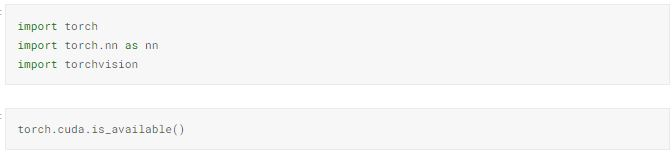
\includegraphics[width=\linewidth]{images/init.JPG}
  \caption{Ukázka kódu třídy pro zařáteční inicializaci}
\end{figure}

Imputs, neboli příprava vstupů. Důležitá součást začátku, zde se nastavuje vše, jak má výsledný model fungovat. Jaké má mít parametry a jaký konkrétní algoritmus se použije pro výpočet. V mém modely je aplikováno 6 modelů. 

\begin{figure}[h!]
  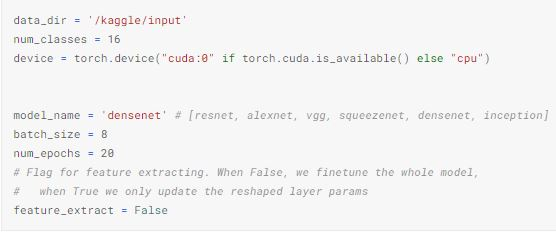
\includegraphics[width=\linewidth]{images/Imputs.JPG}
  \caption{Ukázka kódu třídy pro Přípavu vstupů}
\end{figure}

Ukázka algoritmu, který se bude používat pro výpočet strojového učení. Na konkrétním příkladu je Inception v3. Ale v modelu je aplikováno více algoritmů, které mají podobnou strukturu. 

\begin{figure}[h!]
  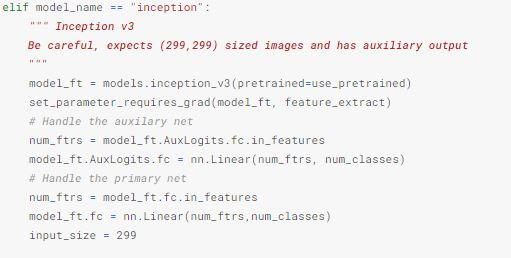
\includegraphics[width=\linewidth]{images/Inception.JPG}
  \caption{Ukázka jedno z algoritmů}
\end{figure}

Ukázka algoritmu z přípravy dat, o které jsem mluvil výše. Dataset se snímky je nejdříve rozdělen do dvou skupin a tyto skupiny jsou následně zpracovány algoritmem. Každá skupina používá jiné metody pro úpravy a zpracování dat. Poté, co proběhne zpracovací část, jsou data načte do paměti a připravena pro následné trénování pomocí neuronových sítí a algoritmu, který jsme si zvolili za začátku. 

\begin{figure}[h!]
  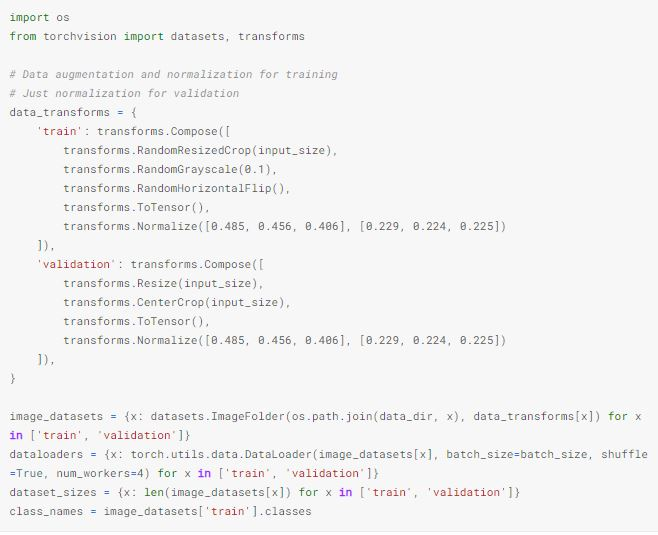
\includegraphics[width=\linewidth]{images/Dataprep.JPG}
  \caption{Ukázka kódu třídy pro přípavu dat}
\end{figure}

Pokud v pořádku a správně proběhnou předchozí kroky můžeme se pustit do samotného učení a trénování. Jak můžeme vidět níže, ukázku z úspěšného trénování. V tomto případě byl použit model inception a celkovým časem 14 minut 29 vteřin a měl nastavených 20 opakovacích cyklů. Výstup je i graf pro lepší orientaci. 

\begin{figure}[h!]
  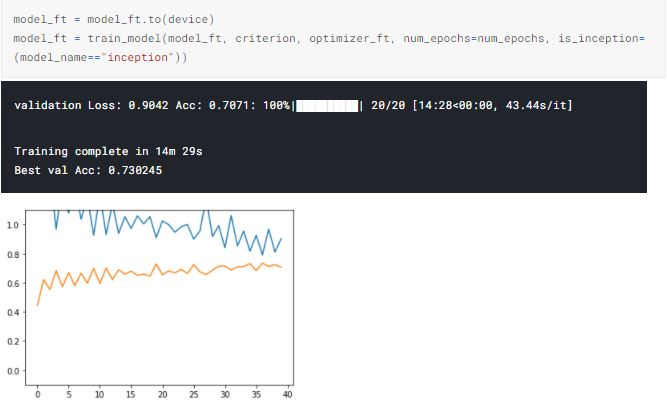
\includegraphics[width=\linewidth]{images/training.JPG}
  \caption{Ukázka trénování neuroných sítí pomocí algorimu}
\end{figure}

Po dokončení trénování a výsledcích modelu, je potřeba tyto výsledky skontroval a poupravit. Pro kontrolu a úpravu výsledků se používá druhá část dat, které jsme si připravili v sekci příprava dat. Data se porovnání oproti nim a popřípadě se upravuje hodnota  plt.pause(0.001). V tomto případě se zvětšuje o 1 tisícinu, tak aby byli výsledky co nejpřesnější mohou být. 

\begin{figure}[h!]
  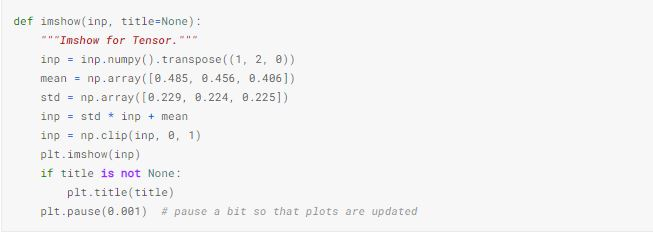
\includegraphics[width=\linewidth]{images/eval.JPG}
  \caption{Ukázka kódu třídy pro kontrolu výsledku}
\end{figure}



\section{TESTOVÁNÍ VYVINUTÉ APLIKACE - ŘEŠENÍ}
Obsah této kapiloly už vypovídá z názvu, bude zda potřeba stavnoti testové scénáře a následně vyhodnotit nově vytvořenou aplikaci.

Testování aplikace na přesnost jednotlivých modelů a času, který na to daný algoritmus potřeboval čili rychlost. Test této funkcionality bude prováděn následně. Do zdrojového kódu budou vždy uloženy stejné výchozí hodnoty pro všechny modely, jediné, co se bude měnit je dan algoritmus. Nastavení hodnot batchsize bude rovno 10 a numepochs bude nastaveno na 20.Dále výsledek bude porovnávám se stejným snímkem a to s vascular2144.png. Pro lepší představu, vyzkoušíme 2 kolový průběh. Po dokončení testu, bude výsledek algoritmu zanesen do tabulky pro porovnání hodnot s ostatními. Tento test bude proveden 1x pro každý model, který aplikace nabízí. Ve výsledku bude test proveden 6x.

\begin{figure}[h!]
  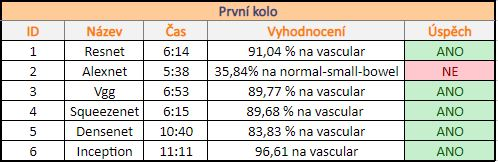
\includegraphics[width=\linewidth]{images/firstround.JPG}
  \caption{První kolo testování algoritmů}
\end{figure}

Z výsledků v prvním kole testů můžeme vidět pár základních věcí. 5 z 6 algoritmů obstály a správně zhodnotili výsledek. U všech výše zmíněných algoritmů se jedná o rozdíly v čase i přesnosti výsledku. Většina algoritmů má rozmezí mezi 80-90 procent úspěšnosti rozpoznání snímku. Nejlepší algoritmus na procentuální skóre se jeví jako Inception, který se svými 96,61 procenty vyhrál náš srovnávací test. Na druhou stranu to zvládl za 11 minut a 11 vteřin. To je nejdelší čas z výše testovaných algoritmů. 

\begin{figure}[h!]
  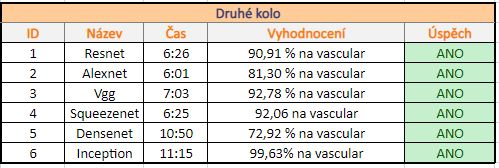
\includegraphics[width=\linewidth]{images/secondround.JPG}
  \caption{Druhé kolo testování algoritmů}
\end{figure}

V druhém kole můžeme vidět zlepší nějaký algoritmů. V tomto kole můžeme říci, že všechny algoritmy dali správný výsledek. Minulé kolo algoritmus Alexnet nesprávně vyhodnotil snímek a určil jsou nemoc na snímku. Druhé kolo přineslo opět stejného vítěze a to Inception, který zvítězil s 99,63 procent a časem 11 minut a 15 vteřin. Algoritmus se o 2 setiny procenta zlepšil, ale časově i o 4 vteřiny pohoršil. 

Porovnání obou našich kol vychází konstantní výsledky většiny algoritmů. Ve druhém kole se nejvíce zlepšil algoritmus Alexnet, který se opravil z prvního kola. Toho je velice důležitý moment, vidíme že je důležité vyzkoušet průběhy algoritmů více než jednou. Absolutním vítězen se stal algortmus Inception, který měl nevyšší procento úspěšnosti odhadu snímku, proti tomu trvalo mu to nejdelší dobu ze všech zmíněných algoritmů. Rozdíly mezi jednotlivými koly nejsou nijak výrazná, kromě jednoho případu. 


\section{CONCLUSIONS / ZÁVĚRY}
Cílem tohoto projektu bylo vytvořit aplikaci na strojové učení, která bude brát jako svůj vstup dataset snímků nemocí. Snímky si sama rozpočítá a pomocí nadefinovaných algoritmů na stojové učení. Poté se začne učit pomocí neuronových sítí. Až se toho vše dokončí porovná se s kontrolní složkou, kterou si aplikace vytvořila v průběhu. Poté nám může prezentovat její výsledek vůči námi vybranému snímku. 

Aplikace byla naprogramována pomocí knihovny Pytorch a pomocí jejich algoritmů. Z provedených testů v tabulkách víše, je patrné že aplikace funguje. Liší se jednotlivé modely a jejich potřeba času na načtení a následné vyhodnocení proti porovnávanému snímku. Samozřejmě se liší i procentuální úspěšnost jednotlivých modelů. Časy jednotlivých modelů se liší o více jednotky minut v našem případě. Oproti tomu, procentuální výsledky nejsou tolik rozdílné a když přihlédneme k času, který potřebujeme na výsledek může se zdát, že algoritmus, který má nejvyšší přenost, nemusí být pro nás ta nejlepší volba. 

Tato aplikace a popřípadě celý model, je demonstrací, že strojové učení může rozhodne fungovat a může být hodně užitečné i v případech lidského zdraví. V případě, že se stane chyba při vyhodnocení špatné marketingové strategie, nemusí to znamenat smrt lidí, nebo v lepším případě zdravotní komplikace jako u biomedicíny. Ke strojovému učení je potřeba přistupovat s pokorou. Je to výborný nástroj do budoucna a myslím, že obliba strojového učení, nebo spíše celého odvětví umělé inteligence jen poroste a více a více aplikací pro běžnou potřebu obyčejného člověka bude napojeno na ty to algoritmy a mnozí lidé o tom nemusí ani vědět. Největší nebezpečí se skrývá v nevědomosti uživatelů a tím, jak je nakládáno s jejich daty. Tento problém se začíná projevovat už v dnešní době. 


% seznam zdrojů
\begin{thebibliography}{1}
\bibitem{}
Pocket-lint. „What Is Apple Deep Fusion and How Does It Work?" Pocket-lint, 29. říjen 2019. https://www.pocket-lint.com/phones/news/apple/149594-what-is-apple-deep-fusion.

\bibitem{}
„Apple’s ‘Neural Engine’ Infuses the IPhone With AI Smarts". Wired. Viděno 13. leden 2021. https://www.wired.com/story/apples-neural-engine-infuses-the-iphone-with-ai-smarts/.

\bibitem{}
SearchEnterpriseAI. „What Is Machine Learning (ML)?" Viděno 14. leden 2021. https://searchenterpriseai.techtarget.com/definition/machine-learning-ML.

\bibitem{}
Kothari, Mahak. „Comparison of Different Deep Learning Models for Image Classification". Medium, 7. duben 2020. https://medium.com/@mahakkothari190.mk/comparison-of-different-deep-learning-models-for-image-classification-1c49f1159d7a.

\bibitem{}
Gao, Xiaohong W., Rui Hui, a Zengmin Tian. „Classification of CT Brain Images Based on Deep Learning Networks". Computer Methods and Programs in Biomedicine 138 (leden 2017): 49–56. https://doi.org/10.1016/j.cmpb.2016.10.007.

\bibitem{}
Chantamit-o-pas, Pattanapong, a Madhu Goyal. „Prediction of Stroke Using Deep Learning Model". In Neural Information Processing, Iconip 2017, Pt V, editoval D. Liu, S. Xie, Y. Li, D. Zhao, a E. S. M. ElAlfy, 10638:774–81. Cham: Springer International Publishing Ag, 2017. https://doi.org/10.1007/978-3-319-70139-478.


\bibitem{}
Jeong, Yeonwoo, Boram Lee, Jae-Ho Han, a Jaeryung Oh. „Ocular Axial Length Prediction Based on Visual Interpretation of Retinal Fundus Images via Deep Neural Network". Ieee Journal of Selected Topics in Quantum Electronics 27, č. 4 (srpen 2021): 7200407. https://doi.org/10.1109/JSTQE.2020.3038845.


\bibitem{}
Oberoi, Archna. „9 Machine Learning Examples from Day-to-Day Life". Viděno 15. leden 2021. https://insights.daffodilsw.com/blog/9-machine-learning-examples-from-day-to-day-life.

\bibitem{}
„15 Machine Learning Examples a Applications To Know | Built In". Viděno 15.leden 2021. https://builtin.com/artificial-intelligence/machine-learning-examples-applications.

\bibitem{}
„27 Incredible Examples Of AI And Machine Learning In Practice". Viděno 15. leden 2021. https://www.forbes.com/sites/bernardmarr/2018/04/30/27-incredible-examples-of-ai-and-machine-learning-in-practice/.

\bibitem{}
„Best Languages For Machine Learning in 2020! | by Himani Bansal | Becoming Human: Artificial Intelligence Magazine". Viděno 14. leden 2021. https://becominghuman.ai/best-languages-for-machine-learning-in-2020-6034732dd242.


\bibitem{}
Shetty, Sunith. „What Is PyTorch and How Does It Work?" Packt Hub, 18. září 2018. https://hub.packtpub.com/what-is-pytorch-and-how-does-it-work/.

\bibitem{}
„What Is Kaggle, Why I Participate, What Is the Impact? | Data Science and Machine Learning". Viděno 14. leden 2021. a.

\bibitem{}
„Colaboratory – Google". Viděno 14. leden 2021. https://research.google.com/colaboratory/faq.html.

\bibitem{}
Oden Technologies. „What Is Model Training". Viděno 14. leden 2021. https://oden.io/glossary/model-training/.

\end{thebibliography}

% nebo

% \bibliographystyle{plain}
% \bibliography{references.bib}{}


% that's all folks
\end{document}